\documentclass{article}
\usepackage[utf8]{inputenc}
\usepackage{graphicx}
\usepackage[spanish]{babel}
\usepackage{amssymb,amsmath,geometry,wrapfig}
\usepackage[hidelinks]{hyperref}
\usepackage{etoolbox} %titulo
\makeatletter %titulo
\patchcmd{\@maketitle}{\vskip 2em}{\vspace*{-3cm}}{}{} %titulo
\makeatother %titulo
\usepackage{vmargin}
\setpapersize{A4}
\setmargins{2.5cm}       % margen izquierdo
{1.5cm}                        % margen superior
{16.5cm}                      % anchura del texto
{23.42cm}                    % altura del texto
{10pt}                           % altura de los encabezados
{1cm}                           % espacio entre el texto y los encabezados
{0pt}                             % altura del pie de página
{2cm}                           % espacio entre el texto y el pie de página
\title{Cicloide}
\author{Aitor Moreno Rebollo y Andoni Latorre Galarraga}
\date{}
%comandos
\newcommand{\bb}[1]{\mathbb{#1}}
\newcommand{\R}{\bb{R}}
\begin{document}
\setlength{\parindent}{0cm}
\maketitle
\section{Descripción}
Si tomamos una circunferencia de radio $r$ y observamos la trayectoria que recorre el punto que comienza en el punto más bajo durante una vuelta completa, obtenemos una cicloide.
\begin{center}\begin{align*}
    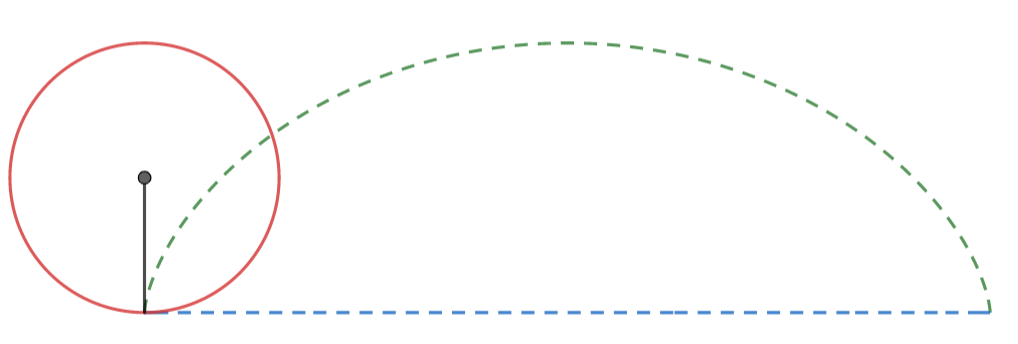
\includegraphics[scale=0.4]{figuras/cicloide descipcion 1.PNG}&
    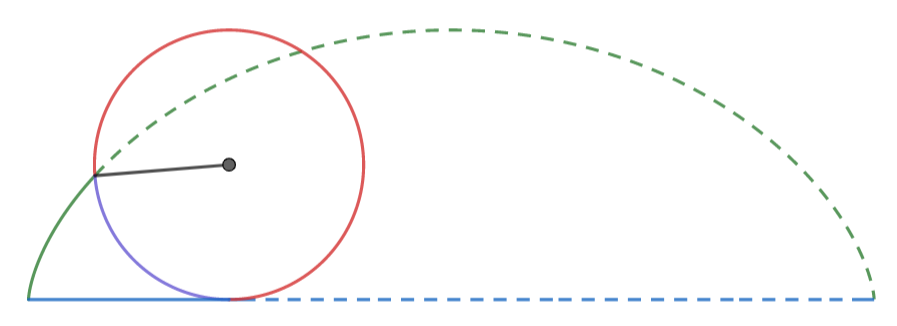
\includegraphics[scale=0.4]{figuras/cicloide descipcion 2.PNG}\\
    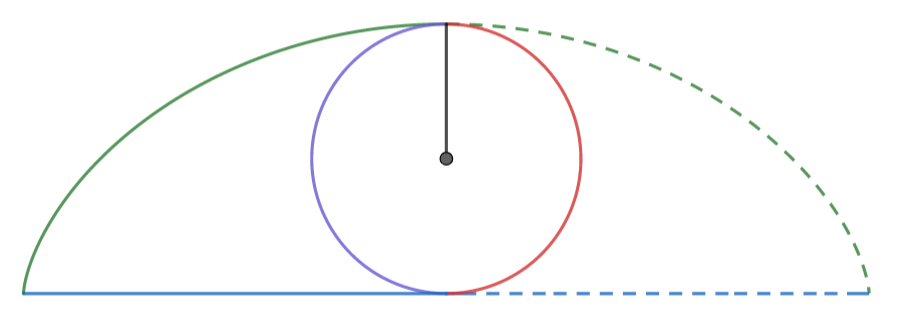
\includegraphics[scale=0.4]{figuras/cicloide descipcion 3.PNG}&
    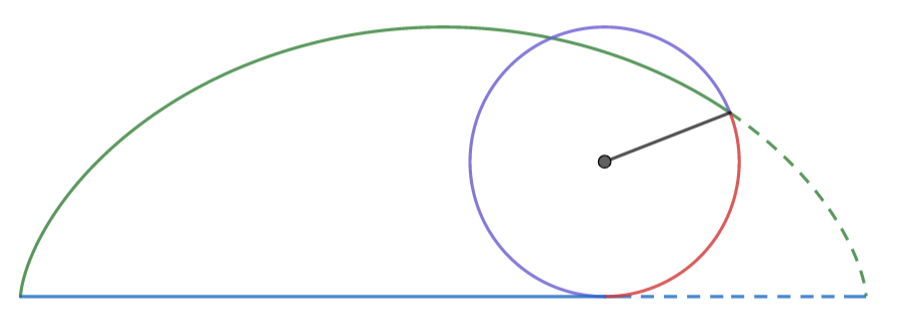
\includegraphics[scale=0.4]{figuras/cicloide descipcion 4.PNG}
\end{align*}
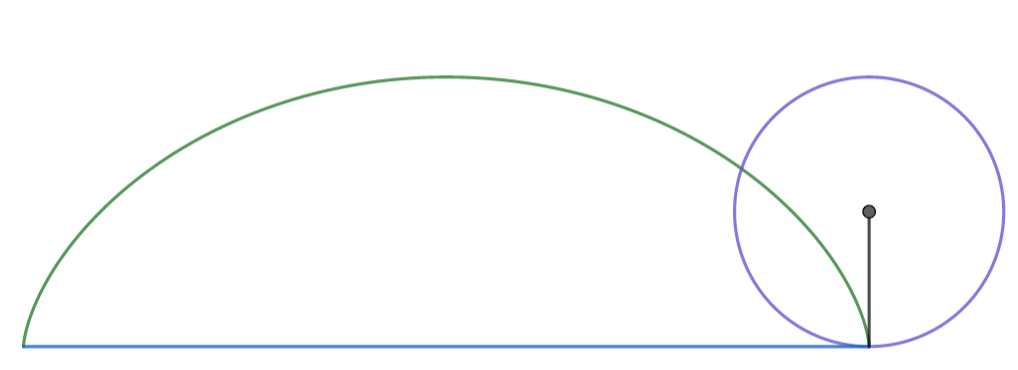
\includegraphics[scale=0.4]{figuras/cicloide descipcion 5.PNG}\\
\href{https://www.geogebra.org/calculator/ju6wnwpc}{Geogebra applet}
\end{center}
\newpage\section{Parametrización}
Partimos de la ecuación de una circunferencia cuyo ángulo sea medido de la siguiente manera:
\begin{center}
        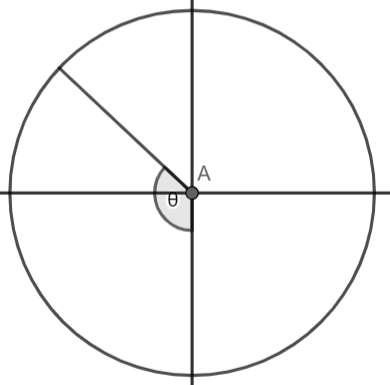
\includegraphics[scale=0.4]{figuras/circulo angulo.PNG}
\end{center} Pues nos resultará idóneo cuando rodemos la circunferencia. Se tiene:\\
$\left\{\begin{array}{lll}
    \theta = 0 & \Rightarrow & \alpha(\theta)=(0,-1) \\
    \theta = \frac{\pi}{2} & \Rightarrow & \alpha(\theta)=(-1,0) \\
    \theta = \pi & \Rightarrow & \alpha(\theta)=(0,1) \\
    \theta = \frac{3\pi}{2} & \Rightarrow & \alpha(\theta)=(1,0)
\end{array}\right.$
y, por tanto la ecuación de esta circunferencia viene dada por $\alpha(\theta)=(-\sen(\theta),-\cos(\theta))$ (si es de radio $1$).
Ahora vamos a suponer que la circunferencia tiene radio $r$; $\alpha(\theta)=r(-\sen(\theta),-\cos(\theta))$.
La ''apoyamos'' en el eje $X$, centrándola en $(0,r)$: $\alpha(\theta)=r(-\sen(\theta),1-\cos(\theta))$.
Ahora vamos a rodarla. Esto lo haremos encontrando una función adecuada $x(\theta)$ tal que la coordenada $x$  del punto avance.
Consideramos $\alpha(\theta)=r(x(\theta)-\sen(\theta),1-\cos(\theta))$, que es la ecuación de la circunferencia cuya coordenada
$x$ va desplazándose acorde con $x(\theta)$. Para lograr la cicloide, debemos hallar $x(\theta)$ tal que $x(\theta)$
''avance al ritmo de la rodada de la circunferencia''. Para ello, consideramos el siguiente esquema:
\begin{center}
    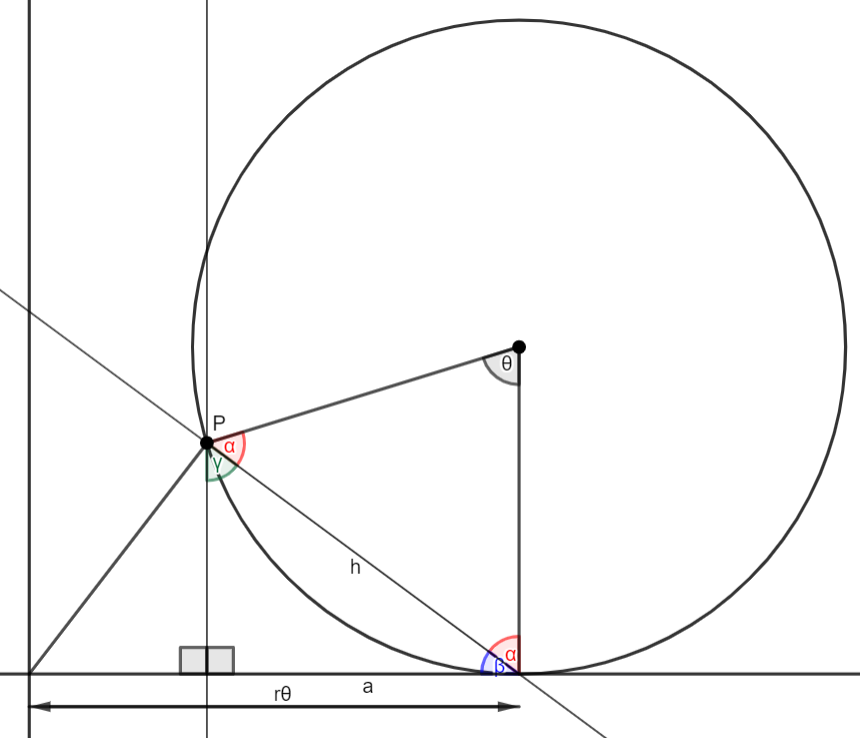
\includegraphics[scale=0.3]{figuras/esquema.PNG}
\end{center}
Sabiendo que la posición del centro de la circunferencia tiene por coordenada $x=r\theta$ (una vez rodado un ángulo $\theta$),
queremos hallar el valor de $a$, pues la coordenada del punto $P$ (genera la cicloide) es $r\theta-a$.
Conociendo el ángulo $\theta$ y el radio $r$, vamos a hallar $a$ en función de $r$ y $\theta$.
$$
\theta + 2\alpha = \pi \: \Rightarrow \: \alpha=\frac{\pi-\theta}{2}
$$
$$
\beta = \frac{\pi}{2}-\alpha
$$
$$
\gamma=\frac{\pi}{2}-\beta=\frac{\pi}{2}-\frac{\pi}{2}+\alpha=\alpha=\gamma
$$
Aplicando el teorema del seno:
$$
\frac{h}{\sen(\theta)} = \frac{r}{\sen \left( \frac{\pi-\theta}{2} \right)} \: \Rightarrow \:
h = \frac{r \sen(\theta)}{\sen \left( \frac{\pi-\theta}{2} \right))}
$$
$$
\frac{a}{h}=\sen(\gamma)= \sen(\alpha)=\sen\left( \frac{\pi-\theta}{2} \right)
$$
$$
a=h\sen\left( \frac{\pi-\theta}{2} \right)= r\sen(\theta)
$$
Por tanto la cicloide tiene la parametrización
$$
\alpha(\theta)=(r\theta-r\sen(\theta),r-r\cos(\theta))
$$
Se nos puede plantear la duda ¿qué ocurriria si en vez de tomar $x(t)=rt$, tomáramos una función distinta?
Es decir, si el punto $P$ que dibuja la cicloide, girara por la circunferencia más rápido o despacio que la rodadura,
en vez de estar fijo. Nos queda una degeneración de la cicloide. Algunas de estas variaciones pueden entenderse también de la
siguiente manera: Habiendo partido de una circunferencia $c(t)=r(-\sen(t),1-\cos(t))=(-r\sen(t),r-r\cos(t))$, de radio $r$
y centrada en $(0,r)$, ¿qué ocurriría si el punto que que dibuja la cicloide estuviera dentro o fuera del círculo? Es decir:\\
\begin{center}
    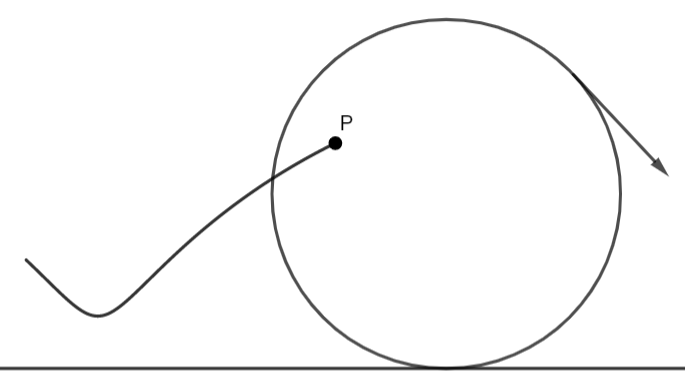
\includegraphics[scale=0.3]{figuras/cicloide general.PNG}
\end{center}
Podemos hacer esto tomando una variación $v$ en el radio de la circunferencia generatriz, quedándonos:
$\alpha(t)=(rt-(r+v)\sen(t),r-(r+v)\cos(t))$ De esta manera, la circunferencia sigue rodando a la vez que $P$, y sigue apoyada en el eje,
pero el punto no está en la propia circunferencia, si no dentro o fuera, dependiendo del signo de $v$:
$$
\begin{array}{ll}
    v>0 & \text{Cicloide alargada} \\
    v<0 & \text{Cicloide acortada}
\end{array}
$$
\begin{center}
    \href{https://www.geogebra.org/calculator/cen7wfhh}{Geogebra applet}
\end{center}
Además pueden generarse muchas otras degeneraciones de la cicloide tomando $x(t)$ como otras funciones cualesquiera,
las cuales pueden forzar a la cicloide a volverse y degenerarse mucho más. También se puede considerar
$\alpha(t)=r(x(t)-f(t)\sen(t),1-f(t)\cos(t))$, donde el punto $P$ varía en su distancia al centro de la circunferencia
tal y como $f(t)$ dicte.\\
Vamos a considerar el caso en el que $P$ está en la circunferencia y el radio es $1$, pues es las cicloide general.
\section{Velocidad}
Tenemos que
$$
\alpha(t) = (t- \sen(t),1-\cos(t))
$$
$\alpha'(t) = (1-\cos(t),\sen(t))$ es el vector tangente.
$$
\left\| \alpha'(t) \right\| = \sqrt{1-2\cos(t)+\cos^2(t)+\sen^2(t)}=\sqrt{2-2\cos(t)}
$$
La circunferencia de partida $\beta(t)=(-\sen(t),-\cos(t))$ tiene $\beta'(t)=(-\cos(t),\sen(t))$ que es $(1,0)+\alpha'(t)$.
Tiene sentido dada la variación de la coordenada $x$ del punto $P$ que genera la cicloide.
\section{Diedro de Frenet}
$$
\alpha''(t)=(\sen(t),\cos(t))
$$
$$
\bb{T}(t)=\frac{\alpha'(t)}{\left\| \alpha'(t)  \right\|} = \left( \frac{1-\cos(t)}{\sqrt{2-2\cos(t)}},\frac{\sen(t)}{\sqrt{2-2\cos(t)}} \right)
= \left( \sqrt{\frac{1-\cos(t)}{2}} , \frac{\sen(t)}{\sqrt{2-2\cos(t)}} \right)
$$
$$
\bb{N}(t) = \mathcal{J}\bb{T}(t)= \left( \frac{-\sen(t)}{\sqrt{2-2\cos(t)}}, \sqrt{\frac{1-\cos(t)}{2}}\right)
$$
$$
k_2(t)=\frac{\alpha''(t)\cdot\bb{N}(t)}{\left\| \alpha'(t) \right\|^2}
=\frac{(\sen(t),\cos(t))\cdot(1-\cos(t),\sen(t))}{(2-2\cos(t))^{\frac{3}{2}}}
=\frac{\sen(t)}{(2-2\cos(t))^{\frac{3}{2}}}
$$
\section{Longitud}
Para calcular la longitud de la cicloide evaluamos la siguiente integral
$$
\int_0^{2\pi} \left\| \alpha'(t) \right\| dt = \int_0^{2\pi} \sqrt{2-2\cos(t)} dt =\sqrt{2} \int_0^{2\pi} \sqrt{1-\cos(t)} dt
$$
$$
= \sqrt{2}\left[ -2 \sqrt{1-\cos(t)}\cot\left(\frac{t}{2}\right)\right]_0^{2\pi} = \sqrt{2}\sqrt{2}4=8
$$
% \subsection{Parametrización por Longitud de arco}
% Primero calculamos la integral
% $$
% \int_0^\theta \left\| \alpha'(t) \right\| dt = \int_0^\theta \sqrt{2-2\cos(t)} dt =\sqrt{2} \int_0^\theta \sqrt{1-\cos(t)} dt
% = \sqrt{2}\left[ -2 \sqrt{1-\cos(t)}\cot\left(\frac{t}{2}\right)\right]_0^\theta 
% $$
% $$
% =\sqrt{2}\left(
% \left(-2 \sqrt{1-\cos(0)}\cot\left(\frac{0}{2}\right)\right)
% -
% \left(-2 \sqrt{1-\cos(\theta)}\cot\left(\frac{\theta}{2}\right)\right)\right)
% $$
% $$
% =\sqrt{2}\left(
% 2 \sqrt{1-\cos(\theta)}\cot\left(\frac{\theta}{2}\right)\right)
% $$
\section{Curiosidades}
\subsection{Curva braquistócrona}
La palabra braquistócrona viene del griego \textit{braquistos} que significa el más corto y \textit{chronos} que significa tiempo,
es decir, la curva que tiene el tiempo más corto. Si tenemos dos puntos $ P $, $ Q $ y queremos encontrar la trayectoria que
minimiza el tiempo de trayecto entre $ P $ y $ Q $. Obtenemos que dicha trayectoria es una cicloide.
\subsection{Curva tautócrona o isócrona}
Las palabras tautócrona e isócrona vienen de los prefijos griegos \textit{tauto/iso} que significan el mismo y de la palabra griega
\textit{choronos} que significa tiempo, es decir, la curva tautócrona o isócrona es aquella en la que no importa el punto de partida,
el tiempo requerido para llegar al punto más bajo es siempre el mismo. De nuevo, dicha curva es una cicloide.
\subsection{Péndulos isócronos}
\begin{center}
    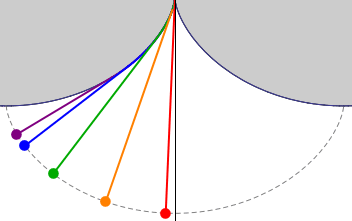
\includegraphics[scale=0.5]{figuras/pend 1.PNG}\\
    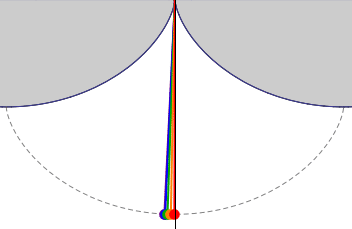
\includegraphics[scale=0.5]{figuras/pend 2.PNG}
\end{center}
Las curvas que se ven en la parte superior son cicloides, de esta manera las cuerdas que sostienen los péndulos van tomando la
forma de parte de la cicloide y otra parte recta. Estos péndulos tienen la propiedad de tener oscilaciones isócronas, es decir,
el tiempo es el mismo.
\end{document}